\section{Обзор предметной области}
\label{sec:domain:intro}

В данном разделе будет произведён обзор программных средств аналогичных разрабатываемому в рамках дипломного проекта - определение психологических параметров человека по образцу почерка, а так же литературных источников. Проанализированы преимущества и недостатки различных подходов к выделению и классификации признаков рукописного текста.

\subsection{Графология}
\label{sub:domain:grafologic}
\emph{Графология} - это учение, постулирующее наличие устойчивой связи месту почерком и индивидуальными особенностями личности.

Идея использования почерка для выявления психологических параметров личности впервые была предложена в 1622 в книге итальянского профессора Камилло Бальдо <<Как узнать природу и качества человека, взглянув на букву, которую он написал>>~\cite{kamillo_grafology}. Первым кто систематизировал знания стал Фландрэна аббат Мишон в 1872 году. Он проанализировал большое количество работ по графологии и образцов почерка и в своей книге <<Система графологии>> предложил \emph{метод Мишона}, он основывался на анализе штрихов, букв, слов, свободных движений, строк и пр.~\cite{mishon_grafology}

Начиная с середины 20 века графология начала рассматриваться как псевдонаучное учение~\cite{graphology_wiki}. По результатам исследования профессиональным графологам не удалось достоверно оценить трудовые способности человека. В среднем профессиональные графологи давали такую же по степени достоверности оценку, как и люди «с улицы»~\cite{neter_shakhar_psevdograph, king_koehler_psevdograph}. В десятках исследований было показано отсутствие связи особенностей почерка с трудовыми способностями человека.

Тем не менее графология широко используется в современной практике отбора кадров~\cite{graphology_psyfactor}.

Основные признаки почерка, которые анализирует графологическая экспертиза:
\begin{enumerate}
  \item размер букв (очень маленькие, маленькие, средние, крупные);
  \item наклон букв (левый наклон, легкий наклон влево, правый наклон, резкий наклон вправо);
  \item направление почерка: (строчки ползут вверх, строчки прямые,  строчки ползут вниз);
  \item размашистость и сила нажима: (легкая, средняя, сильная, очень сильная);
  \item характер написания слов (склонность к соединению букв и слов, склонность к отдалению букв друг от друга, смешанный стиль);
  \item общая оценка (почерк старательный, почерк неровный, почерк небрежный, почерк неразборчивый).
\end{enumerate}

Перечисленные параметры почерка являются устойчивыми, но все же присутствует естественные отклонения параметров (длина, ширина, толщина, угол) от средних значений. Вариация становится наиболее заметной при изменение психологического состояния человека, например при страхе, беспокойстве, алкогольном опьянении.

\subsection{Анализ аналогов}
\label{sub:domain:analogs}

\subsubsection{ScriptAlyzeR}
\label{sub:domain:analogs:neuro_script} 

Программное средство <<ScriptAlyzeR>> является частью семейства программных средств для работы с рукописным текстов компании <<NeuroScript>> и представляет собой дестопное приложение для операционных систем Windows~\cite{analogs_scriptAlyzer}.

Основными возможностями ПС являются:
\begin{itemize}
  \item отслеживание положения, давления, ориентации с частотой 100-200 Гц;
	\item поддержка отслеживания руки, стилуса и мыши;
	\item измеряйте координацию одновременно две рук;
	\item отображение результатов в реальном времени;
	\item изменение толщины линии. Визуальная и звуковая обратная связь;
	\item искажение визуальная обратная связь. Поворот, перекос и отражение на мониторе компьютера в режиме реального времени;
	\item моделирование. Генерация рукописных цифровых данных с шумом и известными характеристиками штрихов;
	\item проверка непротиворечивости.
	\item анализ результатов. Статистика результатов с визуализацией;
	\item многостраничная записи. Разделение текст на слова и штрихи;
	\item внешние приложения. Полная интеграция с вашими собственными модулями с использованием сценариев MATLAB® или скомпилированных программ;
	\item оптически сканированные изображения.
\end{itemize}

Основными недостатками ПС являются:
\begin{itemize}
  \item поддержка только ОС семейства Windows (XP, 7, 8);
  \item платное использование (799+ US\$).
\end{itemize}

Согласно утверждениям разработчиков ПС может быть использовано для оценки моторных функций, диагностики неврологических отклонений, а так же тестирования на состояние алкогольного опьянения.

\begin{figure}[ht]
    \centering
    \label{fig:domain:analogs:neuro_script}
    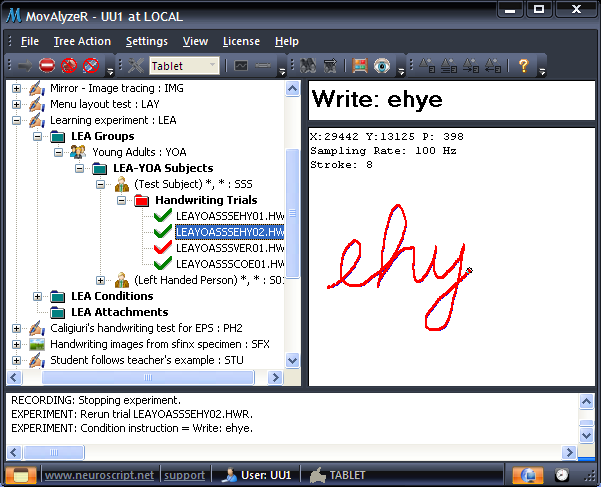
\includegraphics[width=0.7\textwidth]{figures/neuroscript.png}
    \caption{Программное средство <<ScriptAlyzeR>>}
\end{figure}

\subsubsection{Graphology}
\label{sub:domain:analogs:graphology} 

Программное средство <<Graphology>> является приложение для операционной системы Android разработанным компанией <<LH Apps>>~\cite{analogs_graphology}.

Программное средство <<Graphology>> предназначена для анализа почерка и определения характеристик личности. Алгоритм работы программы основан на обширных исследованиях и был создан при консультации профессиональных экспертов графологии.

Основными возможностями ПС являются:
\begin{itemize}
  \item поддержка ОС Android;
  \item многофакторная оценка параметров личности (почерк, подпись, рисунки);
  \item выполнение анализа без доступа в интернет.
\end{itemize}

Основными недостатками ПС являются:
\begin{itemize}
  \item поддержка только ОС Android;
  \item поддержка только английского языка;
  \item для ввода образцов почерка используется экран смартфона, что приводит к искажению в написании символов при низком разрешении и без использование стилуса.
\end{itemize}

\begin{figure}[ht]
    \centering
    \label{fig:domain:analogs:graphology}
    
\includegraphics[width=0.7\textwidth]{figures/graphology_analog.jpeg}
    \caption{Программное средство <<Graphology>>}
\end{figure}

\subsubsection{Signature Analysis}
\label{sub:domain:analogs:signature_analysis} 

Программное средство <<Signature Analysis>> является приложение для операционной системы Android разработанным компанией <<Beyond Consultancy Services>>~\cite{analogs_signature_analysis}.

Программное средство <<Signature Analysis>> предназначена определения характеристик личности по образцу подписи. В разработке участвовал графолог с многолетним опытом, выступающей в качестве консультанта многих крупных компаний.

Основными возможностями ПС являются:
\begin{itemize}
  \item поддержка ОС Android;
  \item широкий спектр анализируемых параметров подписи (скорость, давление, длины, направления);
\end{itemize}

Основными недостатками ПС являются:
\begin{itemize}
  \item поддержка только ОС Android;
  \item платный анализ каждой подписи (0,83 US\$);
  \item для работы необходимо интернет соединение;
  \item для ввода образцов почерка используется экран смартфона, что приводит к искажению в написании символов при низком разрешении и без использование стилуса.
\end{itemize}

\begin{figure}[ht]{}
    \centering
    \label{fig:domain:analogs:signature_analysis}
    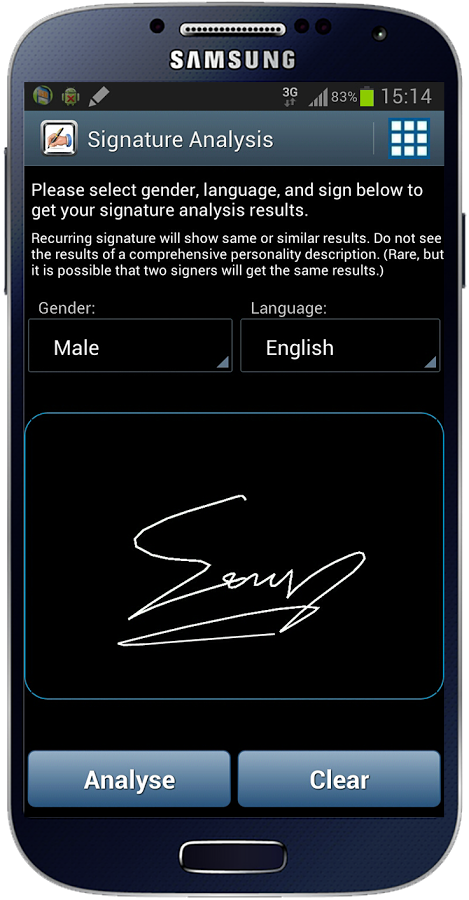
\includegraphics[height=0.4\textheight]{figures/analog_signature_analysis.png}
    \caption{Программное средство <<Signature Analysis>>}
\end{figure}

\subsubsection{My Graphology}
\label{sub:domain:analogs:my_graphology}

Программное средство <<My Graphology>> является приложение для операционной системы Android разработанным компанией <<PENS>>~\cite{analogs_my_graphology}.

\begin{figure}[h]
    \centering
    \label{fig:domain:analogs:my_graphology}
    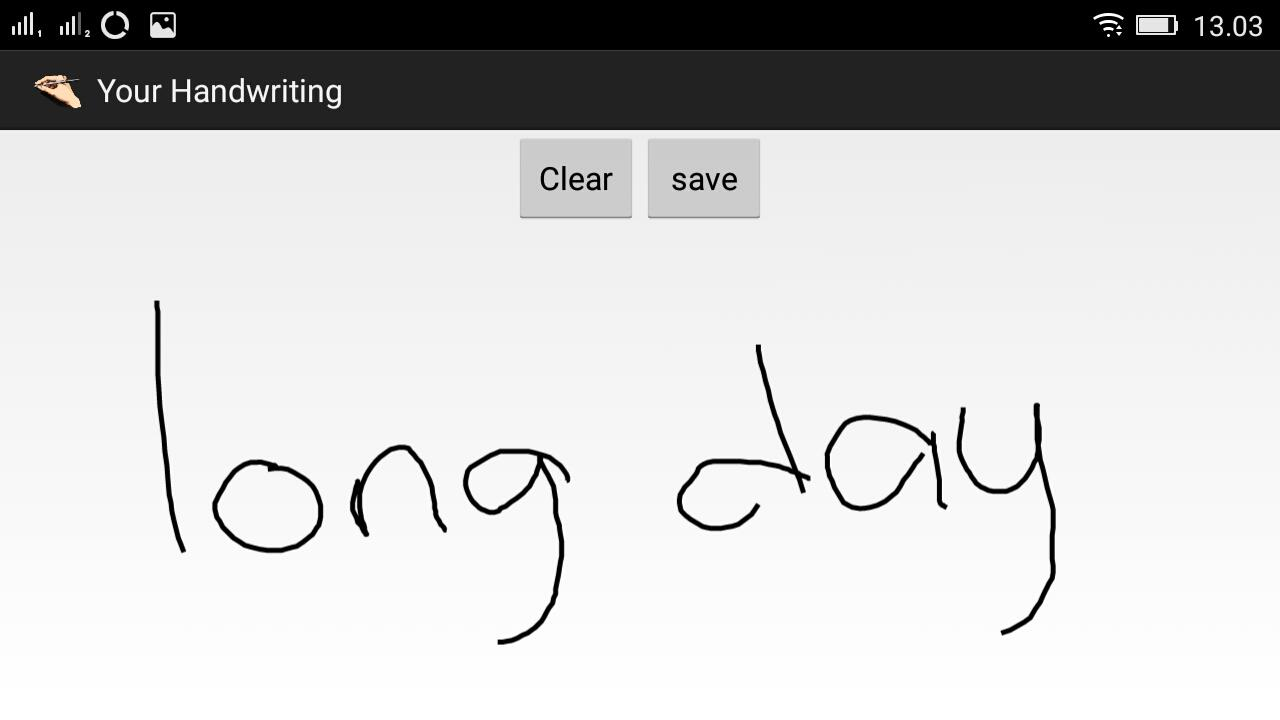
\includegraphics[width=0.4\textheight]{figures/analog_my_graphology.jpeg}
    \caption{Программное средство <<My Graphology>>}
\end{figure}

Основными возможностями ПС являются:
\begin{itemize}
  \item поддержка ОС Android;
  \item использовать для ввода экран или фотографию почерка;
  \item выполнение анализа без доступа в интернет.
\end{itemize}

Основными недостатками ПС являются:
\begin{itemize}
  \item поддержка только ОС Android;
  \item в разработке не участвовали эксперты графологи;
  \item поддержка только испанского языка интерфейса.
\end{itemize}

\subsubsection{GRAPHOLOGY signature analysis}
\label{sub:domain:analogs:graphology_sign_analysis}

Программное средство <<GRAPHOLOGY signature analysis>> является приложение для операционной системы Android разработанным компанией <<DokThor>>~\cite{analogs_graphology_sign_analysis}. Программное средство <<GRAPHOLOGY signature analysis>> предназначена определения характеристик личности по образцу подписи.

\begin{figure}[h]
    \centering
    \label{fig:domain:analog:graphology_sign_analysis}
    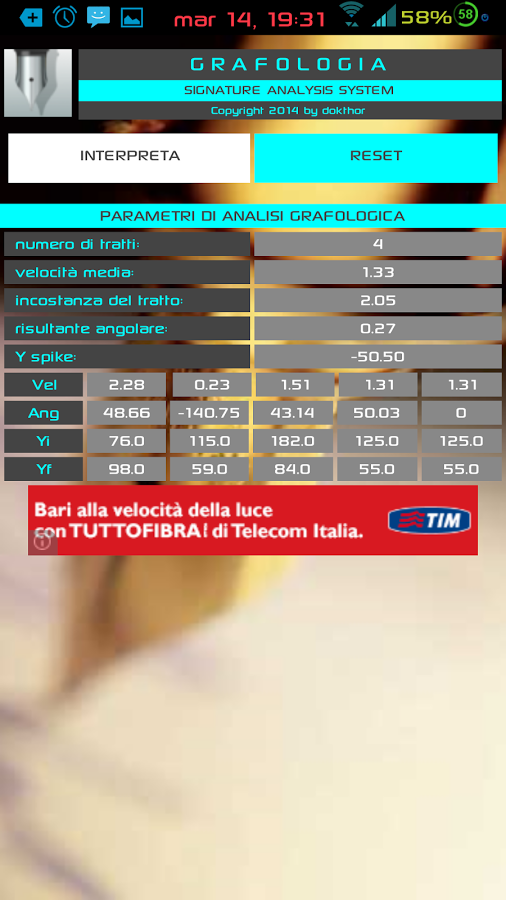
\includegraphics[height=0.5\textheight]{figures/analog_graphology_sign_analysis.png}
    \caption{<<GRAPHOLOGY signature analysis>>}
\end{figure}

Основными возможностями ПС являются:
\begin{itemize}
  \item поддержка ОС Android;
  \item выполнение анализа без доступа в интернет;
  \item предоставление характеристик по личности по 5 основным критериям.
\end{itemize}

Основными недостатками ПС являются:
\begin{itemize}
  \item поддержка только ОС Android;
  \item в разработке не участвовали эксперты графологи;
  \item механизм ввода подписи неочевиден;
  \item для ввода образцов почерка используется экран смартфона, что приводит к искажению в написании символов при низком разрешении и без использование стилуса.
\end{itemize}

\subsubsection{Graphology Lite}
\label{sub:domain:analogs:graphology_lite}

Программное средство <<Graphology Lite>> является приложение для операционной системы Android разработанным компанией <<Hyperborea>>~\cite{analogs_graphology_lite}.

\begin{figure}[h]
    \centering
    \label{fig:domain:analogs:graphology_lite}
    
\includegraphics[height=0.5\textheight]{figures/analog_graphology_lite.png}
    \caption{Программное средство <<Graphology Lite>>}
\end{figure}

Основными возможностями ПС являются:
\begin{itemize}
  \item поддержка ОС Android;
  \item выполнение анализа без доступа в интернет;
  \item использовать для ввода экран или фотографию почерка.
\end{itemize}

Основными недостатками ПС являются:
\begin{itemize}
  \item поддержка только ОС Android;
  \item в разработке не участвовали эксперты графологи;
  \item бесплатная версия позволяет произвести анализ только одного образца. Платная версия стоит 1.05 US\$.
\end{itemize}

\subsection{Анализ литературных источников}
\label{sub:domain:literary_sources}

Публикации и научные статьи на темы схожие с темой данной работы можно условно разделить по следующим признакам:
\begin{itemize}
  \item метод сегментации изображения;
  \item метод классификации признаков изображения.
\end{itemize}

Метод сегментации изображения является неотъемлемой частью алгоритмов обработки рукописного текста, будь это распознавание или анализ. От качества сегментации напрямую зависит качество работы всего алгоритма поэтому выбор метода сегментации является важным этапом.

В рассмотренной литературе предлагаются следующие алгоритмы сегментации рукописного текста:
\begin{itemize}
  \item преобразования Хафа~\cite{louloudis_gatos_pratikakis_halatsis};
  \item нечеткие интервалы~\cite{louloudis_gatos_pratikakis_halatsis};
  \item нечеткий и адаптивный рекурсивный метод наименьших квадратов~\cite{louloudis_gatos_pratikakis_halatsis};
  \item статистические методы (средний интервал между строками)~\cite{gomathi_umadevi_mohanavel};
  \item метод Лоулодиса-Гатоса-Пратикакиса-Халатсиса (LGPH)~\cite{louloudis_gatos_pratikakis_halatsis};
  \item проецирование контуров~\cite{louloudis_gatos_pratikakis_halatsis}.
\end{itemize}

Преобразования Хафа является мощным инструментом компьютерного зрения позволяющим извлекать элементы из изображения. Данный метод позволяет достичь высокой точности сегментации текста, однако требует больших вычислительных затрат в связи с объемом вычислений и использованием тригонометрических функций при вычислении.

Метод рекурсивных нечетких и адаптивных наименьших квадратов, так же как и преобразования Хафа широко используется для выделения областей изображения благодаря высокому качеству работы и устойчивости к шумам и искажениям, однако вычислительная стоимость данных методов велика.

Метод Лоулодиса-Гатоса-Пратикакиса-Халатсиса показывает очень хорошие результаты сегментации и по результатам исследований превосходит по качеству и времени работы все приведенные выше алгоритмы, однако он пока находится в состоянии исследования и не имеет реальных примеров реализации и использования в практических проектах.

Методы проецирования контуров и нечетких интервалов хорошо подходят для распознавания печатного текста, но дают плохие результаты при распознавании рукописного из-за динамически изменяющихся интервалов между символами,строками и словами.

Статические методы основаны на разбиении изображении в зависимости от распределения средней яркости частей изображения, качества работы данных методов ниже чем у преобразований Хафа или рекурсивных методов на основе наименьших квадратов, но время работы намного меньше благодаря меньшему количеству вычислений и быстрым операциям сложению и делению.

В разрабатываемом средстве не требуется высокая точность распознавания, как например для распознавания текста, в то время как программное средство может работа с большим количеством изображений одновременно и быстродействие важно. Исходя из этого в качестве алгоритма сегментации будет использоваться статический метод.

Не менее важным является алгоритм классификации так как именно он будет устанавливать соответствие между параметрами текста и психологическими характеристиками, например силой нажима и степенью наклона символа.

В рассмотренной литературе предлагаются следующие алгоритмы классификации признаков рукописного текста:
\begin{itemize}
  \item нейронные сети~\cite{champa_ananda_kumar_ann, grewal_prashar, gabrani_solomon_dviwe,puri_lakhwani, dang_kumar, kathait_singh};
  \item мешок особенностей~\cite{rothacker_bag_of_features};
  \item метод опорных векторов~\cite{slideshare_khandelwal_garg, gabrani_solomon_dviwe, prasad_singh_sapre};
  \item метод основанный на правилах~\cite{champa_ananda_kumar_rule_base}.
\end{itemize}

Метод основанный на правилах заключается в последовательной проверке соответствия параметров почерка набору правил <<если"=то>>. Как пример можно привести правило "Если строку наклонены влево и сила нажима слабая, то человек пессимист не склонный к выражению эмоций". Данный подход основан только на описание графологических метод, обладает высокой скоростью и не требует обучения. Однако требуется определение границ значений анализируемых параметров, а так же количество правил экспоненциально растет с количеством параметров и их возможных значений, так для двух параметров с тремя значениями каждого понадобиться 9 правил~\cite{champa_ananda_kumar_rule_base}, а для пяти параметров уже 243.

Метод основанный на "мешке особенностей" состоит в составлении "словаря слов" на основе большой базы изображений. Данный словарь будет содержать фрагмент изображения описанный каким-либо дескриптором, например SIFT, и частоту появления этого фрагмента. По сути данный метод рассматривает задачу определения психологических параметров как задачу категоризации. Основными недостатками данного метода является необходимость в сборе и ручной обработке, определения параметров личности экспертами графологами, огромной базы изображений, т.к. все образцы почерка достаточно похожи и сложно выделить отличительные признаки.

Использование нейронных сетей является хорошим решением благодаря способности сети обобщать данные, а использование обратного распространения ошибок позволяет добиться очень хорошего качества распознавания. Однако выбор оптимальной структуры сети и функции активации нейронов является нетривиальной задачей, так же время обучения и распознавания относительно велико.

Метод опорных векторов основан нахождение границы классов максимально удаленной от их экземпляров. К его достоинствам относиться хорошее качество распознавания, высокая скорость обучения и классификации. Однако необходим большой объем обучающей выборки, такой чтобы каждый из возможных наборов признаков встречался хотя бы раз, так же вопрос выбор оптимального типа ядер, схож с выборов функции активации для нейронных сетей.

Поскольку объем обучающей выборки не очень велик ($\sim$ 1200 образцов), а точность классификации нейронных сетей и метода опорных векторов примерно равны, однако скорость обучения и распознавания у опорных векторов выше было принято решение использовать метод опорных векторов для классификации.

\subsection{Обоснование выбора языка и сред разработки}
\label{sec:techs:intro}

Выбор технологий является важным предварительным этапом разработки сложных информационных систем. Платформа и язык программирования, на котором будет реализована система, заслуживает большого внимания, так как множество исследований показали, что выбор языка программирования значительно влияет на производительность труда программистов и качество создаваемого ими кода~\cite[c.~59]{mcconnell_2005}.

На выбор технологий повлияли следующие факторы:
\begin{itemize}
\item программное средство должно быть выполнено в виде клиент"=серверного приложения;
\item разрабатываемое ПО должно работать на операционных системах Linux, MacOS и Windows;
\item разработчик имеет опыт работы с объектно"=ориентированными и функциональными языками программирования.
\end{itemize}

\subsubsection{Язык программирования Scala}
\label{sub:techs:scala}
Scala — мультипарадигмальный, компилируемый, строго типизированный язык программирования, спроектированный кратким и безопасным для простого и быстрого создания компонентного программного обеспечения, сочетающий возможности функционального и объектно-ориентированного программирования~\cite{wiki_scala}.

Scala поддерживает объектно-ориентированную и функциональную парадигмы программирования, но доминирующей является объектно-ориентированная. Язык был выпущен для общего пользования на платформе JVM и .NET, так же создан LLVM-компилятор (Scala Native) и транслятор в JavaScript (ScalaJS).

Отличительные особенности языка Scala:
\begin{itemize}
  \item лаконичность. Код на Scala в средней вдвое короче кода на Java.
  \item открытый исходный код. Код стандартной библиотеки опубликован к открытом доступе на портале GitHub и любой желающий, при наличии желания и способностей, может стать участником проекта.
  \item высокий уровень абстракции. В стандартной библиотеке реализованы большинство типичных операции над строками и коллекциями, в частности итерация по элементам коллекции инкапсулирована в методах map, filter, flatMap. Так же выражение for трансформируется в вызов выше описанных методов, что позволяет использовать в нем пользовательские контейнеры и типы данных. 
  \item платформонезависимость. Код языка компилируется в JVM байт-код и может исполняться на любой платформе поддерживающей JVM.
  \item строгая система типов. Позволяет выявить многое ошибки еще на стадии компиляции.
  \item объектно-ориентированность. Язык поддерживает основные концепции объектно-ориентированного программирование (наследование, инкапсуляция, полиморфизм).
  \item функциональность. Язык поддерживает основные концепции функционального программирование (функции высших порядков, сопоставление с образцов, <<ленивые>> вычисления).
  \item расширяемость. В языке присутствуют механизм (неявные преобразования) позволяющий расширять функционал стандартных классов и сторонних библиотек.
  \item использование Java-кода. Возможно использовать не только библиотеки написанные на Java, но и классы написанные на Java в Scala-проекте, но отсутствует полная обратная совместимость.
  \item широкий набор библиотеки. Стандартная библиотека Scala содержит классы для работы с вводом-выводом, регулярными выражениями, параллельной обработки, работы со строками, коллекции. Так же существует большое количество сторонних библиотек.
\end{itemize}

Основываясь на выше перечисленных факторах было принято решение использовать в качестве основного языка программирования Scala как современный, активно набирающий популярность язык поддерживающий функциональную и объектно"=ориентированную парадигмы программирования.

Далее приводится подробная характеристика языка программирования.

\paragraph{Объектно-ориентированное программирование}
Объектно-ориентированная парадигма программирования играет в языке важную роль. Стандартная библиотека языка реализована в виде набора классов и примесей, а так же модульность обеспечивается классами и пакетами~\cite{horsman_scala}.

Особенности Scala с точки зрения объектно"=ориентированной парадигмы:
\begin{itemize}
  \item статическая сильная полная типизация с автоматическим выведением типов;
  \item наследование, в том числе использование примесей (Traits);
  \item полиморфизм;
  \item инкапсуляция;
  \item конструкторы, деструкторы;
  \item все операторы (+, -, *) являются методами;
  \item гибкое управление доступом к полям и методам;
  \item метапрограммирование;
  \item объекты компаньоны (используются для инкапсуляции статических полей и методов).
\end{itemize}

\paragraph{Функциональное программирование}
Особенности Scala с точки зрения функциональной парадигмы:
\begin{itemize}
  \item функции высших порядков;
  \item функции объект первого класса;
  \item оптимизация хвостовой рекурсии;
  \item сопоставление с образцов;
  \item поддержка неизменяемых структур данных;
  \item функциональные комбинаторы и композиции;
  \item частичное применение функции;
  \item <<ленивые>> вычисления;
  \item структурное переиспользование неизменяемых коллекций.
\end{itemize}

\subsubsection{Фреймворк Akka}
\label{sec:techs:akka}

Akka - набор прикладных библиотек (фреймворк) предоставляющий высокоуровневый интерфейс для разработки, развертывания и отладки систем акторов.

Основными достоинствами фреймворка Akka являются:
\begin{itemize}
  \item простота интерфейса, высокая степень абстракции;
  \item устойчивость к отказам. Благодаря механизму супервизор;
  \item масштабируемость. Проста добавления акторов в систему и развертывания компонентов на другой машине;
  \item высокая скорость работы и степень параллелизма. Благодаря использованию модели акторов;
  \item минимально количество блокирующих операций. Отсутствие общего изменяемого состояния.
\end{itemize}

Перечисленные достоинства, в особенности устойчивой к отказам и простота масштабирования, являются крайне важными при реализации архитектуры на основе микросервисов. Исходя из выше перечисленного для обеспечения параллельной обработки данных будет использоваться набор прикладных библиотек (фреймворк) Akka. 

\begin{figure}[ht]
    \centering
    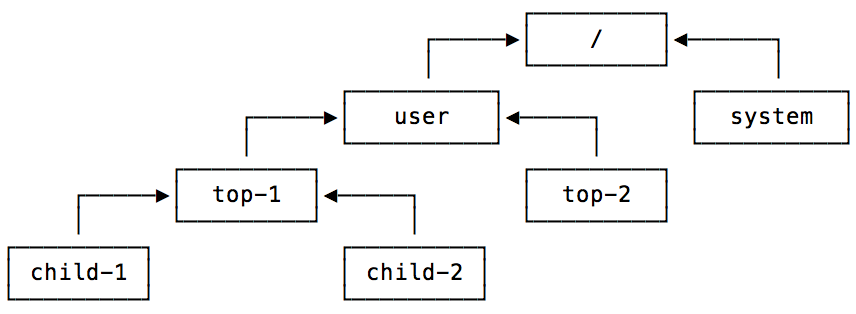
\includegraphics[width=0.7\textwidth]{figures/actors_hier.png}
    \label{fig:techs:akka:actor_hierar}
    \caption{Иерархия акторов}
\end{figure}

\paragraph{Модель акторов}
\label{sec:techs:akka:actor_model}
Модель акторов - модель параллельных вычислений, основанная на взаимодействии изолированных примитивов взаимодействующих по средствам получения и отправки сообщений. Впервые была предложена в 1973 году~\cite{hewitt_bishop_steiger_actor_model}.

Основным понятием данной модели является «актор». Согласно модели актор лишен состояния и информации о структуре системы (количество братьев и родителей). 

\begin{figure}[ht]
    \centering
    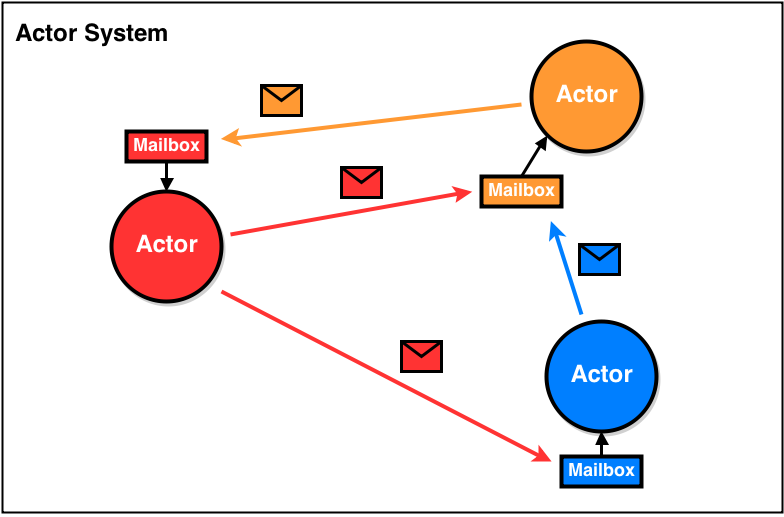
\includegraphics[width=0.7\textwidth]{figures/actor_model.png}
    \label{fig:techs:akka:actor_model:comulication}
    \caption{Пример взаимодействия акторов}
\end{figure}

При получении сообщения актор может:
\begin{itemize}
  \item отправить конечное число сообщений другим акторам;
  \item создать конечное число новых акторов;
  \item выбрать поведение, которое будет использоваться при обработке следующего полученного сообщения.
\end{itemize}

Данный подход позволяет теоретичеки полностью избежать блокировок благодаря отсутсвию прямых вызовов методов актора и даже механизма ожидания ответа.

\subsubsection{Фреймворк Spray}
\label{sec:techs:spray}

Spray - набор прикладных библиотек (фреймворк) предназначенного реализации веб-приложений.

Данный фреймворк базируется на описанном выше фреймворке Akka и реализует асинхронное распределение запросов пользователя на иерархию акторов. 

Основными достоинствами фреймворка Spray являются:
\begin{itemize}
  \item полная асинхронность, отсутствие блокировок (весь интерфейс полностью асинхронный);
  \item высокая производительность (используются специальные низкоуровневые компоненты);
  \item модульность (весь интерфейс полностью асинхронный);
  \item легковесность (включаются только необходимые модули);
\end{itemize}

Использование данного фреймворка позволит упростить разработку, отладку и последующее сопровождения благодаря использования одной концепции с предыдущим фреймворком.
Исходя из выше перечисленного для реализации серверной часть приложения будет использоваться набор прикладных библиотек (фреймворк) Spray.

\subsection{Постановка задачи}
\label{sec:domain:requirements}
В результате анализа было выявлено что текущие аналоги не обладают следующими возможностями необходимыми для эффективного практического использования:
\begin{itemize}
  \item поддержка ОС Linux и MacOS;
  \item поддержка русского языка интерфейса;
  \item взимание платы за использование;
  \item поддержка механизма контроля доступа.
\end{itemize}

В результате выполнения дипломного проекта должно быть разработано программное средство определения психологических параметров личности по образцу почерка, реализующее процедуры выделения признаков почерка из изображения и их классификацию, а так же механизм авторизации для обеспечения секретности данных. К разрабатываемому программному средству предъявляются следующие требования:
\begin{itemize}
\item разрабатываемое ПО должно работать на операционных системах Linux, MacOS и Windows;
\item программное средство должно быть выполнено в виде клиент"=серверного приложения;
\item программное средство должно поддерживать русский язык интерфейса;
\item программное средство должно поддерживать работу как в режиме выделения признаков рукописного текста, так и в режиме их классификации;
\item программное средство должно предусматривать механизм регистрации, аутентификации и авторизации пользователей.
\end{itemize}